\documentclass[10pt,twocolumn]{article}

\usepackage[margin=0.65in,top=0.70in,bottom=0.70in]{geometry}
\usepackage{amsmath}
\usepackage{amssymb}
\usepackage{booktabs}
\usepackage{graphicx}
\usepackage{microtype}
\usepackage{hyperref}
\usepackage{parskip}
\setlength{\parskip}{1.5pt}
\setlength{\intextsep}{4pt}
\setlength{\floatsep}{4pt}
\setlength{\textfloatsep}{4pt}

\hypersetup{colorlinks=true, linkcolor=blue, citecolor=blue, urlcolor=blue}

\title{\textbf{NLI-Based Knowledge Coverage as a Swarm Evaluation Metric}}
\author{}
\date{}

\begin{document}

\maketitle
\vspace{-1.5em}



% -------------------------------------------------------------------------
\section{Experiment Overview}

The system places a swarm of $N$ autonomous agents in a bounded 2-D
environment seeded with \emph{subject} agents, each carrying a short
textual snippet describing a real-world scene (a university career fair).
Agents perform a continuous random walk; upon entering the proximity radius
of a subject they absorb its snippet, and upon meeting a peer they exchange
their current summaries. An LLM fuses the accumulated observations into a
single evolving natural-language summary for each agent.

The central research question is whether, and how quickly, a swarm
collectively acquires a complete, accurate representation of the scene,
and how different communication strategies (self-learning only vs.\
social learning) affect that process. Answering this requires a metric
that can compare an agent's free-form summary against a structured set of
ground-truth facts in a semantically meaningful way, motivating the
NLI-based coverage score described below.

% -------------------------------------------------------------------------
\section{Natural Language Inference and the DeBERTa-v3 Cross-Encoder}

Natural Language Inference (NLI) is the task of determining, given a
\emph{premise} $p$ and a \emph{hypothesis} $h$, whether $p$ entails $h$,
contradicts $h$, or is neutral with respect to $h$~\cite{bowman2015snli}.
We use the \texttt{cross\nobreakdash-encoder/nli\nobreakdash-deberta\nobreakdash-v3\nobreakdash-large}
model~\cite{he2021debertav3}, which concatenates the premise and hypothesis
into a single input sequence and passes it through a DeBERTa-v3-large
encoder. A linear classification head followed by a softmax layer produces
a three-class probability distribution over
$\{\text{contradiction},\,\text{entailment},\,\text{neutral}\}$.

The model is used via the Sentence-Transformers
\texttt{CrossEncoder} API~\cite{reimers2019sentence}.
Given a batch of $(p, h)$ pairs, \texttt{CrossEncoder.predict} returns an
array of softmax probabilities with a fixed index convention:
%
\begin{align}
  \mathbf{p}(p, h) &=
  \bigl[p_{\text{contra}},\; p_{\text{ent}},\; p_{\text{neut}}\bigr]
  \;\in\; \mathbb{R}^{3}, \notag \\
  &p_{\text{contra}} + p_{\text{ent}} + p_{\text{neut}} = 1.
  \label{eq:nli-output}
\end{align}

% -------------------------------------------------------------------------
\section{Coverage Score: Formal Definition}

\subsection{Inputs}

Let $\sigma$ denote the current natural-language summary produced by an
agent, and let
$\mathcal{C} = \{c_1, c_2, \ldots, c_n\}$
be the ground-truth claim set for the current experiment scenario. The
claims are fixed short sentences drawn from a curated library (e.g.\
\emph{``Event staff scan registrations and hand out lanyards at the
entrance.''}) that collectively describe the scene the agents are
exploring.

\subsection{Sentence Tokenization}

The agent summary $\sigma$ is split into individual sentences using
NLTK's Punkt sentence tokenizer, yielding
%
\begin{equation}
  \mathcal{S}(\sigma) = \{s_1, s_2, \ldots, s_m\},
  \label{eq:sent-tok}
\end{equation}
%
where $m = |\mathcal{S}(\sigma)|$ varies with summary length.

\subsection{Pair Matrix Construction}

To check whether the summary supports any given claim, every summary
sentence is paired with every claim. The full set of evaluation pairs is
%
\begin{equation}
  \mathcal{P}(\sigma, \mathcal{C})
  \;=\;
  \bigl\{\,(s_i,\, c_j)\;\bigm|\; s_i \in \mathcal{S}(\sigma),\;
  c_j \in \mathcal{C}\,\bigr\}.
  \label{eq:pair-matrix}
\end{equation}
%
The matrix has $|\mathcal{P}| = m \times n$ entries, enumerated in
\emph{claim-major} order: for each claim $c_j$ all $m$ sentence
counterparts are listed consecutively. The complete batch $\mathcal{P}$
is passed to the NLI model in a single forward pass.

\subsection{NLI Score Matrix}

Applying the model to $\mathcal{P}$ yields a probability matrix
%
\begin{equation}
  \mathbf{P} \;\in\; \mathbb{R}^{n \times m \times 3},
  \qquad
  \mathbf{P}_{j,i} = \mathbf{p}(s_i,\, c_j),
  \label{eq:score-matrix}
\end{equation}
%
where each entry $\mathbf{P}_{j,i}$ is the three-class softmax vector
defined in Eq.~\eqref{eq:nli-output}, with $s_i$ as premise and $c_j$ as
hypothesis.

\subsection{Entailment Decision Per Claim}

For each claim $c_j$ we ask: does at least one sentence in the summary
constitute a premise that unambiguously entails $c_j$? This is answered by
a hard \emph{argmax} decision across the three output classes for every
sentence–claim pair:
%
\begin{equation}
  \hat{\ell}_{j,i}
  \;=\;
  \operatorname*{arg\,max}_{k \;\in\; \{0,1,2\}}
  \mathbf{P}_{j,i}^{(k)},
  \label{eq:argmax}
\end{equation}
%
where $k=1$ corresponds to the entailment class. A claim $c_j$ is
considered \emph{covered} if the entailment label wins for at least one
sentence:
%
\begin{equation}
  \mathrm{covered}(c_j, \sigma)
  \;=\;
  \bigvee_{i=1}^{m}
  \Bigl[\hat{\ell}_{j,i} = 1\Bigr].
  \label{eq:covered}
\end{equation}
%
Using the argmax hard decision avoids introducing a free probability
threshold and is consistent with standard NLI evaluation
practice~\cite{bowman2015snli}.

\subsection{Coverage Score}

The final coverage score is the fraction of ground-truth claims that are
covered by the summary:
%
\begin{equation}
  \boxed{
  \mathrm{Cov}(\sigma, \mathcal{C})
  \;=\;
  \frac{1}{n}
  \sum_{j=1}^{n}
  \mathbf{1}\!\left[\mathrm{covered}(c_j, \sigma)\right]
  \;\in\; [0, 1].
  }
  \label{eq:coverage}
\end{equation}
%
A score of $0$ means the summary entails none of the ground-truth claims;
a score of $1$ means every claim is entailed by at least one sentence of
the summary.

% -------------------------------------------------------------------------
\section{Application in the Swarm System}

\subsection{Agent Behaviour and Summary Formation}

Each \texttt{knowledgeAgent} performs a random walk across a 2-D
continuous environment. Two interaction modes drive knowledge accumulation:
%
\begin{itemize}
  \item \textbf{Subject encounter.} When the agent enters the proximity
    radius of an information site (a \emph{subject} agent), the site's
    textual snippet is appended to the agent's private context buffer
    $\mathbf{p}$ (a bounded deque of capacity $K_p$).
  \item \textbf{Peer encounter.} When two knowledge agents meet, each
    appends the other's latest summary to its received-context buffer
    $\mathbf{t}_{\mathrm{recv}}$ (capacity $K_r$).
\end{itemize}
%
After either interaction, an LLM prompted as a \emph{data-fusion module}
merges the agent's prior summary $\tau_{\mathrm{prev}}$, its private
context, and any received summaries into an updated summary:
%
\begin{equation}
  \tau \;\leftarrow\;
  \mathrm{LLM}\!\left(\tau_{\mathrm{prev}},\;\mathbf{p},\;
  \mathbf{t}_{\mathrm{recv}}\right).
  \label{eq:llm}
\end{equation}
%
The output is capped at 150 words per prompt instruction.

\subsection{Snapshot Evaluation}

The simulation environment records a snapshot every $\Delta t$ seconds.
At snapshot time $t \in \{t_1, t_2, \ldots, t_T\}$, each agent $a$'s
current summary $\sigma_a(t)$ is evaluated:
%
\begin{equation}
  \mathrm{score}_a(t)
  \;=\;
  \mathrm{Cov}\!\left(\sigma_a(t),\,\mathcal{C}\right).
  \label{eq:per-agent}
\end{equation}

% -------------------------------------------------------------------------
\section{Illustrative Result}

\begin{figure}[h!]
  \centering
  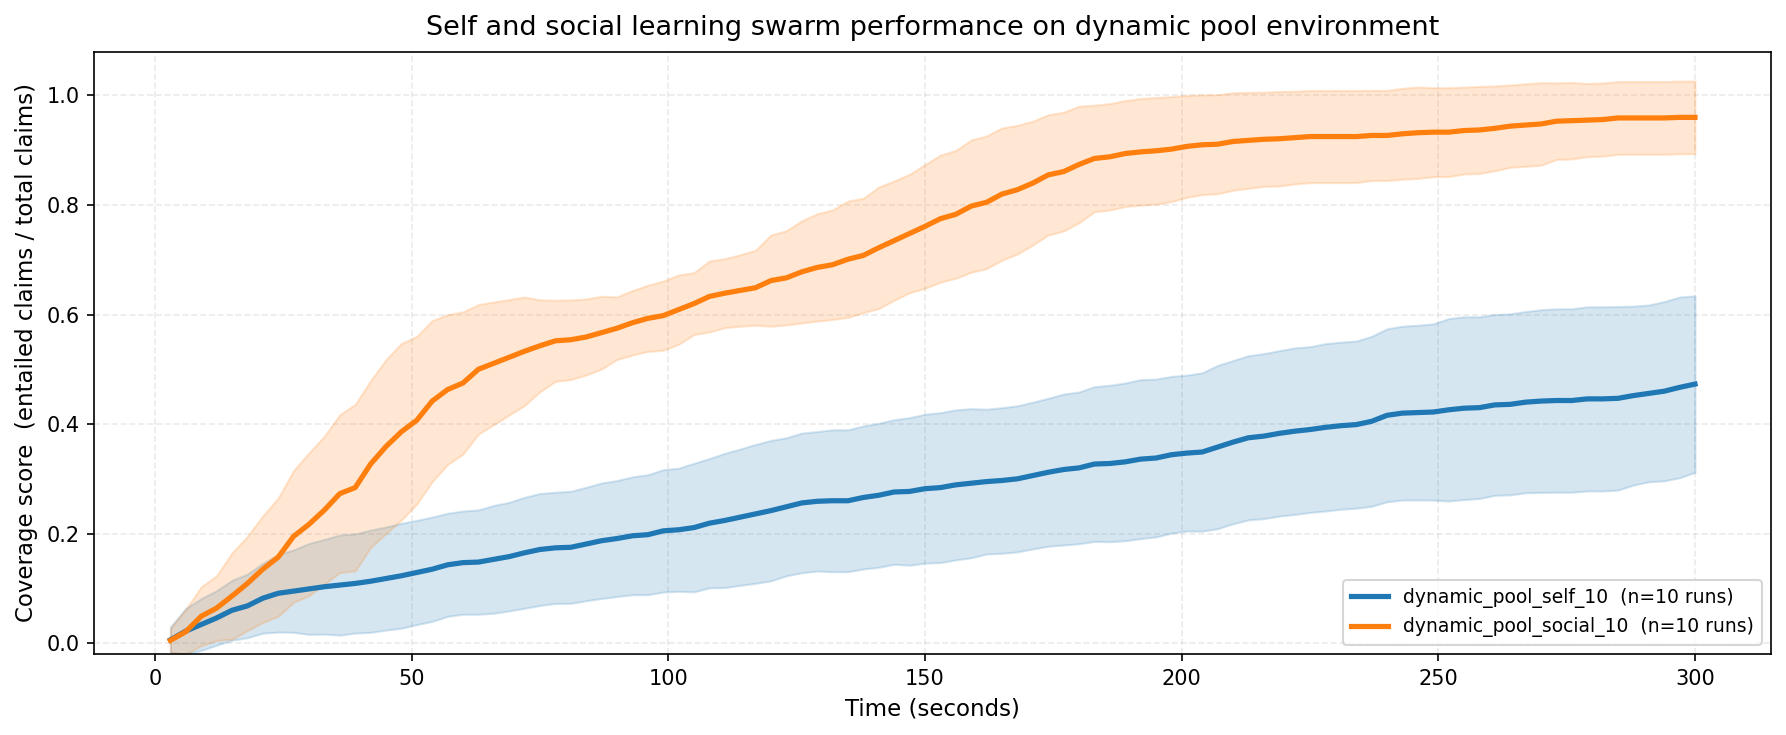
\includegraphics[width=\columnwidth]{dynamic_pool_self_vs_social.png}
  \caption{Average coverage score over time: self-learning vs.\ social
    learning, averaged across $R{=}10$ runs (dynamic-pool environment).}
  \label{fig:self-vs-social}
\end{figure}

Figure~\ref{fig:self-vs-social} plots the swarm-mean coverage
$\bar{S}(t)$ for two experimental configurations in the dynamic-pool
environment. Social learning consistently outpaces self-learning, reaching
near-complete ground-truth coverage within 200 seconds while the
self-learning swarm plateaus below 0.5, demonstrating the metric's
sensitivity to inter-agent communication.

% -------------------------------------------------------------------------
\begin{thebibliography}{9}

\bibitem{bowman2015snli}
S.~R. Bowman, G.~Angeli, C.~Potts, and C.~D. Manning,
``A large annotated corpus for learning natural language inference,''
in \emph{Proc.\ EMNLP}, 2015, pp.\ 632--642.

\bibitem{he2021debertav3}
P.~He, J.~Gao, and W.~Chen,
``DeBERTaV3: Improving DeBERTa using ELECTRA-style pre-training with
gradient-disentangled embedding sharing,''
\emph{arXiv:2111.09543}, 2021.

\bibitem{reimers2019sentence}
N.~Reimers and I.~Gurevych,
``Sentence-BERT: Sentence embeddings using Siamese BERT-networks,''
in \emph{Proc.\ EMNLP}, 2019, pp.\ 3982--3992.

\end{thebibliography}

\end{document}
